\subsection{Zielsetzung und architektonische Anforderungen}
Der Stand der Technik aktueller Simulationsplattformen für Roboter zeigt, dass
virtuelle Steuerungen und damit zusammenhängende Simulationsplattformen
herstellerspezifisch entwickelt und mit Ausnahme von ROS keine einheitliche
Schnittstelle zur Kommunikation mit externen Plattformen oder Physik-Engines
bieten. Somit muss für jeden Robotertyp ein designierter Konnektor genutzt
werden, um diesen mit einer externen, herstellerunabhängigen Simulationplattform
zu verbinden. Um eine herstellerunabhängige und erweiterbare Plattform zu
entwickeln, sollte also eine gemeinsame Schnittstelle implementiert werden.\\

\noindent
Zusammenfassend verfolgt die Architektur des Frameworks drei zentrale Ziele:
\begin{enumerate}
	\item \textbf{Vendor-Agnostik}: Abstraktion verschiedener Roboterhersteller durch einheitliche Interface-basierte Architektur ohne herstellerspezifische Abhängigkeiten im Kern-Framework

	\item \textbf{Modulare Erweiterbarkeit}: Plugin-System für Safety Monitoring Module und Kommunikationsprotokolle ohne Änderungen der bestehenden Architektur

	\item \textbf{Echtzeitfähige Kommunikation}: Latenzarme Datenübertragung für Motion Control und ereignisbasierte Sicherheitsüberwachung
\end{enumerate}

\subsection{Unity3D als Simulationsplattform}

Die Wahl von Unity3D als zugrundeliegende Simulationsplattform basiert auf
mehreren technischen und praktischen Erwägungen. Während es bereits mehrere
kommerzielle Programme für die Gestaltung und Simulation von Robotern in
virtuellen Umgebungen gibt, sind diese nur selten mit anderen CAD-Systemen und
Robotern kompatibel, unterstützen nicht alle Roboterbibliotheken oder werden
nur plattformabhängig angeboten (vgl. \vglcite[247]{andaluz2016}). Unity3D
hingegen ist mit den meisten CAD-Systemen kompatibel und bietet eine
plattformübergreifende Lösung.\\

\noindent
Unity3D bietet eine ausgereifte 3D-Rendering-Pipeline mit integrierter
Physik-Engine, welche zur Simulation von Gegenständen mit realitätsnahem
Verhalten sowie komplexen Arbeitsräumen geeignet ist \vglcites{\cite@single{Unity2025SystemRequirements};\cite@single{Unity2025PhysicsOverview}}.
Die Engine wurde bereits erfolgreich in der wissenschaftlichen Forschung
eingesetzt und bietet Module und Plugins für spezifische Anwendungsfälle im
Simulationsbereich. Unity3D ermöglicht es auch Nicht-Programmierern,
leistungsstarke Animations- und Interaktionsdesign-Tools zu nutzen, um Roboter
visuell zu programmieren und zu animieren vgl. \vglcite[431]{bartneck2015}.\\

\noindent
Technisch ermöglicht Unity3D durch seine Scripting-Runtime (basierend auf
Mono/.NET Framework) die Verwendung moderner C\#-Sprachfeatures für
nebenläufige Prozesse und asynchroner Programmierung
\vglcite[45-52]{unity_async_2023}, was es ermöglicht, Visualisierung,
Datenakquise und Überwachung zu trennen. Die .NET-basierte Architektur
unterstützt dabei sowohl Task-basierte asynchrone Operationen als auch
Coroutines für zeitgesteuerte Prozesse
\vglcite[123-135]{unity_coroutines_2023}, welche die notwendige periodische
Ausführung von Prozessen auf verschiedenen Ebenen des Frameworks stark
vereinfacht.\\

\noindent
in weiterer Vorteil für die Robotik-Simulation liegt in der
Verfügbarkeit visueller Programmiertools und der integrierten
Entwicklungsumgebung. Die Plattform bietet umfangreiche Debugging- und
Profiling-Werkzeuge (Unity Profiler, Frame Debugger), die während der
Entwicklung und zur Laufzeit genutzt werden können
\vglcite[S.~67-89]{unity_profiler_2023}. Diese Werkzeuge ermöglichen die
Analyse von Performance-Engpässen bei der Verarbeitung von Roboterdaten und die
Optimierung der Sicherheitsmonitor-Updates.

Darüber hinaus lassen sich während der Laufzeit sowohl die Szene (hier: die
Roboterzelle) als auch Komponenten-Parameter in Echtzeit bearbeiten und
einsehen \vglcite[1236]{haas2022}, was das Debuggen und Testen
beschleunigt.

\subsection{Design Patterns und Prinzipien}

Die Entwicklung eines modularen und erweiterbaren Robotersicherheitssystems
erfordert eine fundierte methodische Herangehensweise, die auf bewährten
Software-Engineering-Prinzipien basiert. Die Auswahl geeigneter Design Patterns
und Architekturprinzipien determiniert maßgeblich die Qualitätsattribute des
Systems wie Wartbarkeit, Testbarkeit und
Erweiterbarkeit.\vglcite[73\psqq]{Bass2012} Im Folgenden werden die für diese
Arbeit gewählten Entwurfsmuster und deren Begründung dargelegt.

Für die Realisierung der systemweiten Kommunikation wird das Observer
Pattern\vglcite[293-303]{Gamma1994} als zentrales Entwurfsmuster gewählt. Diese
Entscheidung basiert auf einer zentralen Überlegung: Zunächst muss gewährleistet sein,
dass alle relevanten Ereignisse an relevante Systemkomponenten weitergegeben
werden. Daher ermöglicht das Muster die dynamische Registrierung
und Deregistrierung von Beobachtern zur Laufzeit\vglcite[127\psq]{Buschmann1996} Drittens
reduziert die lose Kopplung zwischen Publisher und Subscriber die
Systemkomplexität erheblich, da Komponenten ohne Kenntnis voneinander
interagieren können.


Die Vorteile dieser Architekturentscheidung manifestiert sich vornehmlich
darin, dass so Robotertypen ohne Modifikation des Kernsystems integriert
werden. \textsc{Martin2003} spricht hier vom Open-Closed-Prinzip, welches die
Offenheit von Software-Entitäten (Funktionen, Klassen, Module, Komponenten
usw.) zur Extension und die gleichzeitige Geschlossenheit zur Modfikation
beschreibt.\vglcite{Martin2003}

\subsubsection{Adapter Pattern zur Hardware-Abstraktion}
Die Integration heterogener Hardware-Komponenten erfordert eine
Abstraktionsschicht zwischen der Anwendungslogik und den hardware-spezifischen
Schnittstellen. Das Adapter Pattern (vgl. \vglcite{Gamma1994}, S. 139-150) wird
gewählt, um diese Abstraktion zu realisieren. Die Notwendigkeit ergibt sich aus
der Vielfalt der Robotersteuerungen und Visualisierungssysteme, die jeweils
eigene APIs und Datenformate verwenden (vgl. \vglcite{Craig2005}, S. 412-415).

Durch die Adapter-Schicht wird eine einheitliche Schnittstelle zur Verfügung
gestellt, die es ermöglicht, verschiedene Robotersysteme ohne Änderung der
Kernlogik anzubinden. Dies reduziert nicht nur die Komplexität des Systems,
sondern erhöht auch dessen Portabilität und Wiederverwendbarkeit (vgl.
\vglcite{Vlissides1995}, S. 89-91).

\subsubsection{SOLID-Prinzipien als Qualitätsfundament}
Die konsequente Anwendung der SOLID-Prinzipien \vglcite{Martin2003} bildet das methodische Fundament der Systemarchitektur. Das
\textit{Single Responsibility Principle} wird angewendet, um kohäsive Module zu
schaffen, die genau eine Verantwortlichkeit haben. Dies reduziert die Kopplung
und erhöht die Verständlichkeit des Codes \vglcite{Martin2017}. Das \textit{Open-Closed Principle} gewährleistet, dass das System für
Erweiterungen offen, aber für Modifikationen geschlossen ist – eine essenzielle
Eigenschaft für langlebige Industriesysteme.

Das \textit{Dependency Inversion Principle} wird konsequent angewendet, indem
High-Level-Module von Abstraktionen abhängen, nicht von konkreten
Implementierungen. Dies ermöglicht die flexible Konfiguration des Systems zur
Laufzeit und vereinfacht die Integration in verschiedene Produktionsumgebungen
\vglcite[112\psqq]{Fowler2018}

\subsubsection{Event-Driven Architecture für Echtzeitfähigkeit}
Die Entscheidung für eine event-getriebene Architektur basiert auf den
Echtzeitanforderungen industrieller Robotersysteme. Sicherheitskritische
Ereignisse müssen innerhalb definierter Zeitschranken verarbeitet werden, was
durch synchrone Aufrufketten nicht gewährleistet werden kann
\vglcite[97\psqq]{Hohpe2003}. Die event-getriebene Architektur ermöglicht die
asynchrone Verarbeitung von Ereignissen und die Priorisierung kritischer
Sicherheitsereignisse.

Zudem adressiert dieser Ansatz die Herausforderung der Integration verschiedener
Datenquellen – von zyklischen Sensordaten über sporadische Alarme bis zu
kontinuierlichen Videoströmen. Jede Datenquelle kann Events in ihrem eigenen
Takt generieren, ohne andere Systemkomponenten zu blockieren
\vglcite[234\psqq]{Vernon2013}.

\section{Schichtenarchitektur des Frameworks}

Aufbauend auf den oben genannte Prinzipien
teilt sich das Framework in 4 logisch getrennte Module auf:

\begin{enumerate}
	\item \textbf{Kernlogik}, welches den Status des Roboters beinhaltet und
	      verwaltet als zentrale Schnittstelle (Core)\item \textbf{Interfaces},
	      welche die Kommunkationsschnittstellen und -methoden zwischen den Modulen
	      implementiert (Interfaces) \item \textbf{Monitoring}, welches die einzelnen
	      Komponenten des Monitoring-Systems implementiert (Monitors) \item
	      \textbf{Adapters}, welches potenziell Adapter zu veschiedenen physischen oder
	      simulierten Steuerungen von Robotern beinhaltet (Hier ABB gennant)
\end{enumerate}



\begin{figure}[H] \centering
	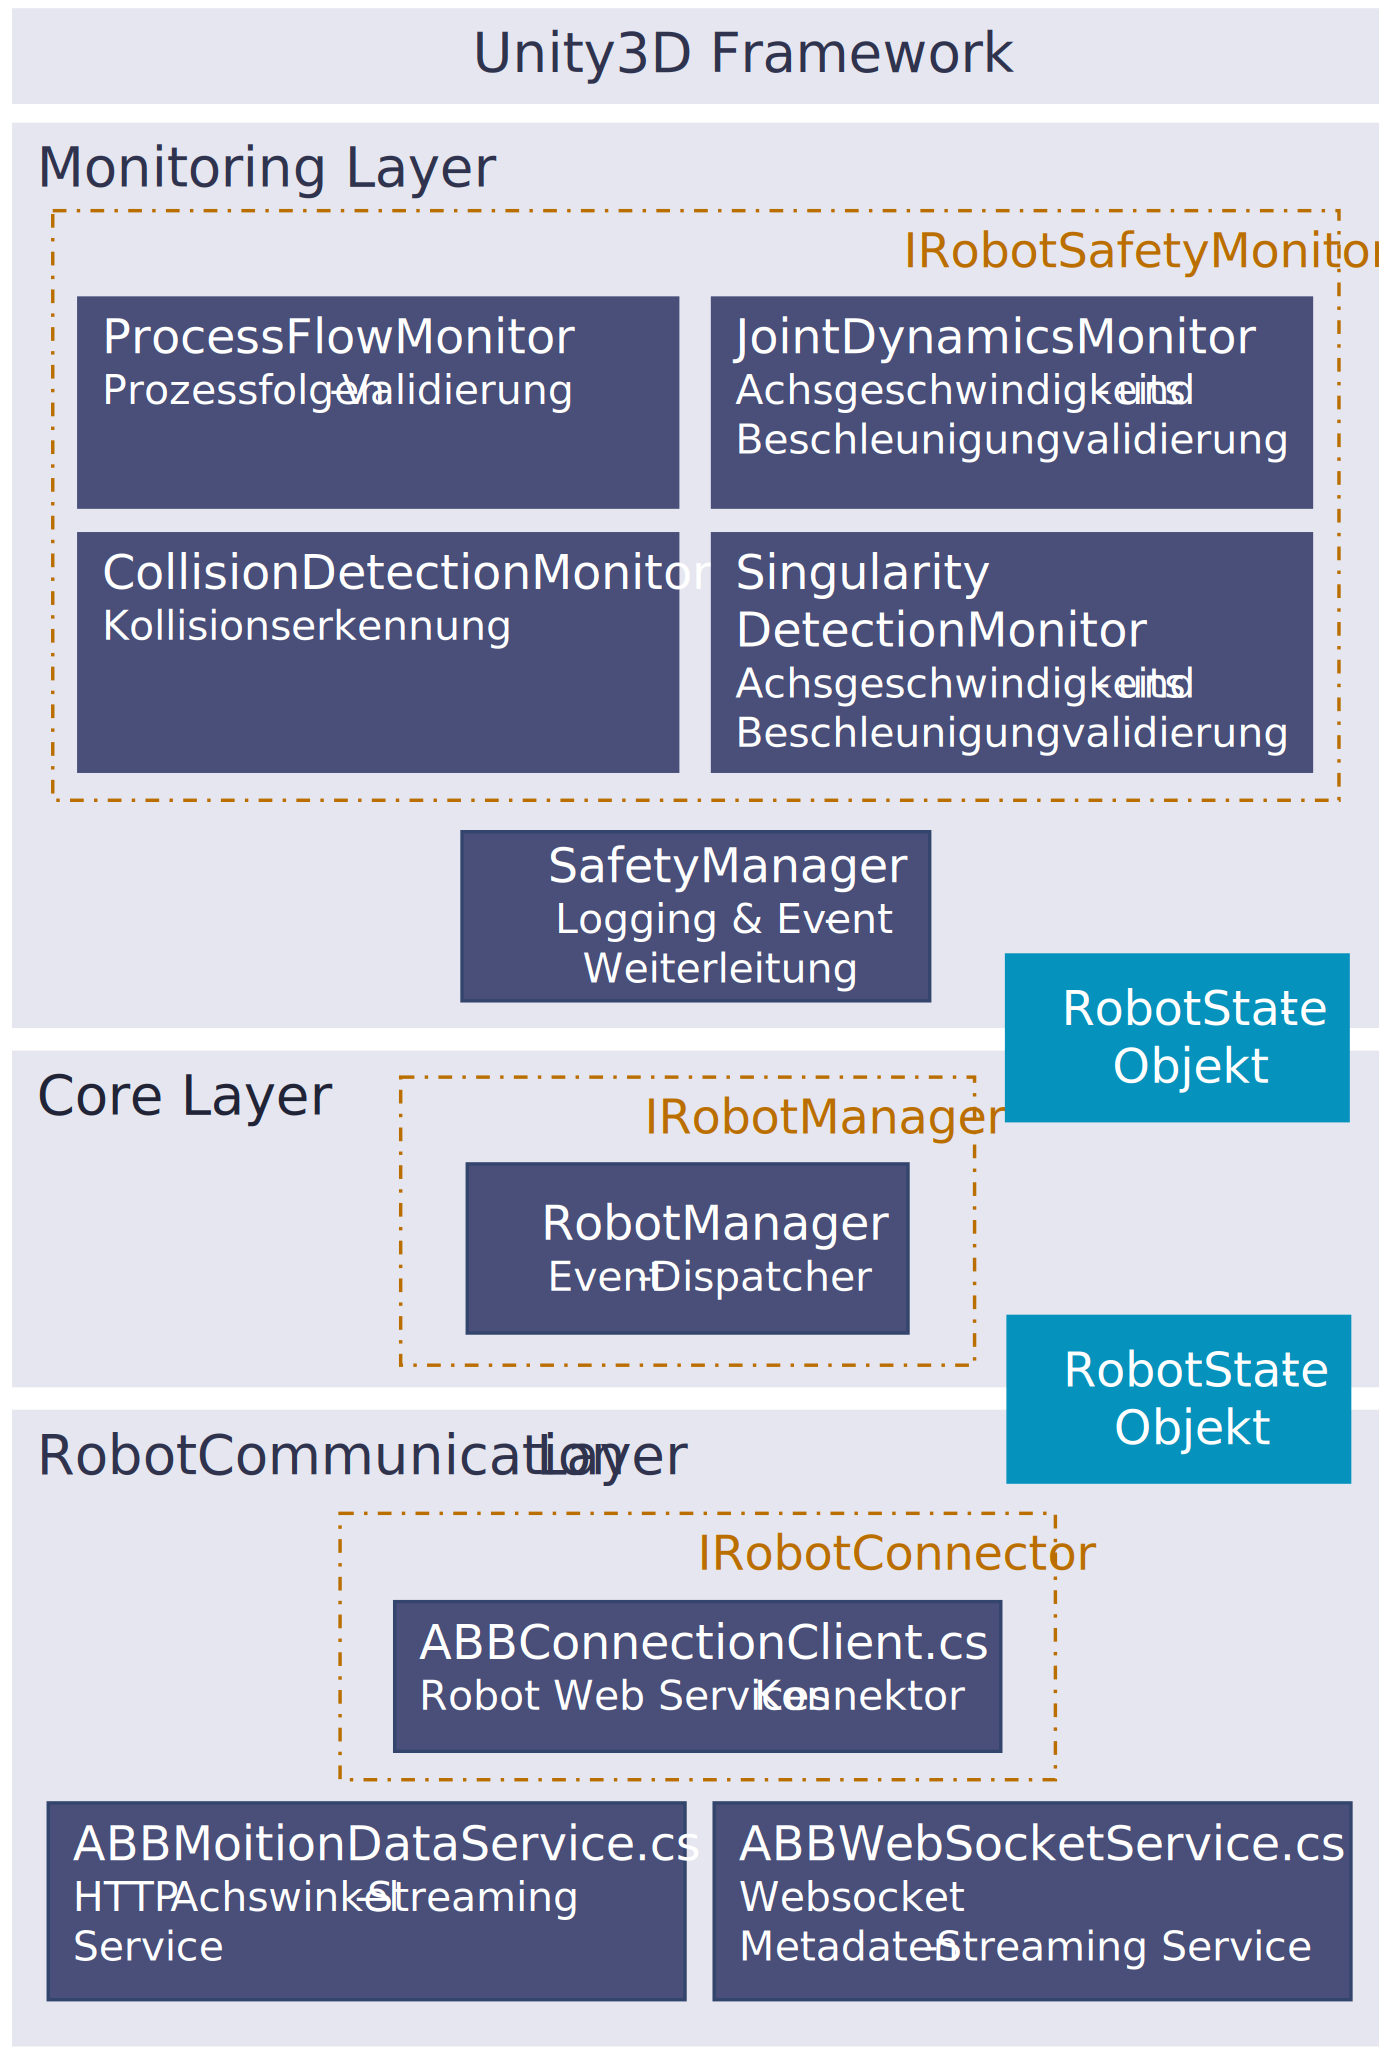
\includegraphics[width=10cm]{Figures/LayerArchitekturFramework.png}
	\caption{Schichtenarchitektur des Frameworks mit den wichtigsten zugehörigen
		Modulen. Module mit grüner Umrandung werden durch eine Interface formalisiert}
	\label{figure:layer}
\end{figure}

Die Trennung der Module ermöglicht eine formalisierte
Schnittstellenkommunikation, dargestellt in Abbildung \ref{figure:layer}.
Jede Schicht hat verschiedene Verantwortlichkeiten und Schnittstellen innerhalb
des Monitoring-Systems. Zentrales Element des Systems stellt der RobotManager
dar. Er dient als Bindeglied zwischen den Monitoring-Komponenten, welche für die
Überwachung des Systems verantworlich sind und der Adapter-Schicht,
verantwortlich für die Kommunikation und das Spiegeln des Roboters aus der
initialen Umgebung (hier RobotStudio) in Unity.

\subsection{Robot Communcation Layer}
Die Robot Communication Layer organisiert die Kommunkation mit der zugrundeliegenden Robotersteuerung und
implentiert eine Interface des Typs IRobotConnector. Als Verbindungsclient
zwischen Unity und externer Schnittstelle des Robotersystems implementiert
dieser eine IRobotConnector Interface, welche als Vorlage für eine Anbindung an
eine Robotersteuerung jedes Typs fungiert und standartisierte Methoden
implementiert:

\begin{figure}[H]
	\inputminted[fontsize=\footnotesize]{csharp}{code-snippets/IRobotConnector.cs}
	\caption{Implementierung der IRobotConnector-Interface als Verbidung zwischen
		RobotState und Roboter-Controller}
\end{figure}
\noindent
Eine Interface lässt sich anhand dieses Beispiels in \textbf{3
	Funktionsbereiche} aufteilen: Events, Attribute und Methoden.\\

\noindent
Die Interface definiert \textbf{Events (Aktionen)} die bei definierten Zustandsänderungen
in der Laufzeit ausgeführt werden. Andere Bestandteile des Framework sind in der
Lage, ein Event zu abonnieren und eine Methode registieren, welche ausgeführt
werden soll, wenn dieses Event auftritt. Ist dies der Fall, wird das
entsprechende Modul über die Änderung benachrichtigt und bekommt gegebenfalls
neue Daten zur Verfügung gestellt. Diese event-getriebene Kommunikation sorgt
dafür, dass einerseits alle Komponenten proaktiv auf den neusten Stand der Daten gebracht
und gehalten werden, andererseits aber keine ressourcenblockierenden Prozesse
ausgeführt werden müssen, um gegebenfalls Statusänderungen abzufragen.\\

\noindent
Weiterführend definiert die Interface IRobotConnector \textbf{Attribute}, welche den
aktuellen Verbindungsstatus (verbunden = \texttt{true}, getrennt = \texttt{false}) speichern sowie das
State-Objekt des Roboters. Definiert durch die schreibgeschützten, automatisch
implementierte Eigenschaft mit einem Getter \textit{\{ get; \}} können Attribute
auch von ausserhalb des RobotConnectors abgefragt werden, jedoch nicht
überschrieben.\\

\noindent
Zuletzt gibt die Interface die Methoden \textit{\textbf{Connect}} und \textit{\textbf{Disconnect}}
vor, welche hier die wichtigsten Methoden zum Verbinden und
Trennen von der jeweiligen Robotersteuerung darstellen.

Als initiale Komponente wird eine Verbindung zum
Controller eines Roboters benötigt, um den Roboter in Unity emulieren zu können
und Daten zu verarbeiten. Dazu wird hier mittels eines HTTP-Clients zur
Schnittstelle des RobotStudioSDKs über die API RobotWebServices (RWS) eine
Verbindung aufgebaut. Die Verbindung zu RobotWebServices ensteht durch einen
HTTP-Client und der Authentifizierung mit in RobotStudio festgelegten
Zugangsdaten. Anschliessend kann über einen erhaltenen Cookie die Verbindung
aufrecherhalten werden und aktuelle Daten über den Roboter sowohl abgefragt,
also auch der Roboter selbst gesteuert werden.\vglcite{robotwebservices2025}

Die RWS-Schnittstelle bietet einerseits die Möglichkeiten,
aktuellen Achswinkel und TCP-Werte (Tool Center Point) abzurufen, als auch
weitere Metadaten, wie das aktuell laufende Programm, den aktuellen Motorstatus
oder auch die Codezeile, welche aktuell vom Programmzeiger ausgeführt wird.
Weiterführend bietet RWS die Möglichkeit, die aktuelle digitale und analoge
Signale abzurufen, was nötig ist, um den Greifer steuern zu können.

Bei den oben genannten Daten mit Ausnahme der Achswinkel handelt es sich um
Paramenter, welche sich im Laufe eines Programmablaufs vergleichsweise selten
verändern. Daher wird hier auf den Websockets-Endpunkt von RWS zugegriffen, um
innerhalb einer Duplex-Kommunikation sich verändernende Signale oder auch
Programmstati zu empfangen. Dazu wird mithilfe des HTTP-Clients eine Anfrage zur
Subscription auf verschiedene Parameter (bspw. den ProgrammPointer) gestellt,
und anschliessend eine Websockets-Session aufgebaut. Die Achswinkel werden
zeitgleich über eine asynchron endlosen Task in einer in Unity definierbaren
Frequenz abgefragt.

Der Client implementiert dabei die Interface IRobotConnector und gibt ein
RobotState-Objekt mit den empfangenen Daten an den RobotManager weiter, welcher hier
als zentraler Koordinator des aktuellen RobotState fungiert.

\noindent
\paragraph{Event-Driven Architecture}
as System nutzt ein durchgängiges Event-System für lose Kopplung:
\begin{itemize}
	\item \texttt{OnRobotStateUpdated}: Zustandsänderungen
	\item \texttt{OnConnectionStateChanged}: Verbindungsstatus
	\item \texttt{OnSafetyEventDetected}: Sicherheitsereignisse
	\item \texttt{OnMotorStateChanged}: Motorstatusänderungen
\end{itemize}

\paragraph{SafetyEvent und RobotStateSnapshot}
Als für die Auswertung der Simulationsergebnisse relevantes Teil des Frameworks
wird eine SaftetyEvent-Objekt implementiert. Jedes Mal, wenn ein Ereignis,
welches mit der tatsächlichen Simluation eines Roboterpgrogramms zusammenhängt,
auftritt, wird ein SafetyEvent instanziert. Dieses wird initial von der
jeweiligen überwachenden Komponente (einem SafetyMonitor) instanziert und mit
dem aktuellsten RobotState als unveränderliches Objekt (RobotStateSnapshot) befüllt.
Weiterführend erhält es vom jeweiligen SafetyMonitor variierende
Kontextinformationen, die später für die Auswertung des Ereignisses verwendet
werden. Zusammenfassend bestehn ein SafetyEvent aus folgenden Komponenten:
\begin{itemize}
	\item \textbf{SafetyEvent}: Unveränderliches Value Object für Sicherheitsereignisse
	\item \textbf{RobotStateSnapshot}: Immutable Zustandserfassung zum Ereigniszeitpunkt
	\item \textbf{Ereignistypen}: Info, Warning, Critical mit konfigurierbaren Schwellwerten
	\item \textbf{Kontextdaten}: Vollständige Roboterzustandserfassung für Forensik
\end{itemize}
\noindent

\dirtree{%
	.1 RobotSystem/.
	.2 Core/.
	.3 RobotManager.cs.
	.3 RobotState.cs.
	.3 RobotSafetyManager.cs.
	.3 SafetyEvent.cs.
	.3 RobotStateSnapshot.cs.
	.3 Part.cs.
	.3 Station.cs.
	.3 RapidTargetGenerator.cs.
	.2 Interfaces/.
	.3 IRobotConnector.cs.
	.3 IRobotDataParser.cs.
	.3 IRobotSafetyMonitor.cs.
	.3 IRobotVisualization.cs.
	.2 ABB/.
	.3 RWS/.
	.4 ABBRWSConnectionClient.cs.
	.4 ABBRWSDataParser.cs.
	.4 ABBMotionDataService.cs.
	.3 ABBFlangeAdapter.cs.
	.2 Monitors/.
	.3 CollisionDetectionMonitor.cs.
	.3 JointDynamicsMonitor.cs.
	.3 ProcessFlowMonitor.cs.
	.3 SingularityDetectionMonitor.cs.
}

s
